\documentclass{beamer}

\usetheme[department=compute]{DTU}

\usepackage[orientation=landscape,size=a1,scale=1.2,debug]{beamerposter}             

\usepackage{multicol} % This is so we can have multiple columns of text side-by-side
\columnsep=100pt % This is the amount of white space between the columns in the poster
\columnseprule=3pt % This is the thickness of the black line between the columns in the poster


\usepackage[T1]{fontenc}
\usepackage[utf8]{inputenc}
\usepackage{lmodern}
\usepackage[english]{babel}
%\usepackage{pgfplots}
%\pgfplotsset{compat=1.9}
%\usepackage{booktabs}
\usepackage{siunitx}


\title{Leverage based sampling for classification }
\author{Julian Kopka Larsen and Jesper Løve Hinrich}
\institute{DTU Compute}

\newcommand{\tabitem}{{\color{dtured}$\bullet$} }
\newenvironment{pblock}{\begin{minipage}[b]{\linewidth}
	\begin{block}}{\end{block} 	\end{minipage}\vspace*{15pt}}
\newcommand{\imblock}[1]{
\includegraphics[width=\linewidth]{#1}}

\begin{document}
\frame{
	\frametitle{Leverage based sampling for classification}
\begin{columns}[t]
    \begin{column}{.3\linewidth}



	\begin{block}{Abstract}
	We validate the results of leverage based sampling for LS-regression, shown by Ma et al. [1]. We explore the possibility of using the leverage based sampling distribution from LS-regression on 2 class classification, and introduce two new approaches for sampling form an leverage distribution (important points).
	\end{block}
	
	\begin{pblock}{Motivation}
	The importance of sampling methods are initiated by very large datasets where it is not feasible to use all of the available data. This is illustrated by the rise in online access to video data. These data contain many frames that are basically the same and therefore redundant. 
	\end{pblock}

	\begin{pblock}{Research Questions}	
	\begin{itemize}
	\item Will the regression based sampling distribution improve our performance in classification?
	\item Can leverage based sampling be generalized to classification?
	\end{itemize}
	\end{pblock}


	\begin{pblock}{Datasets}
	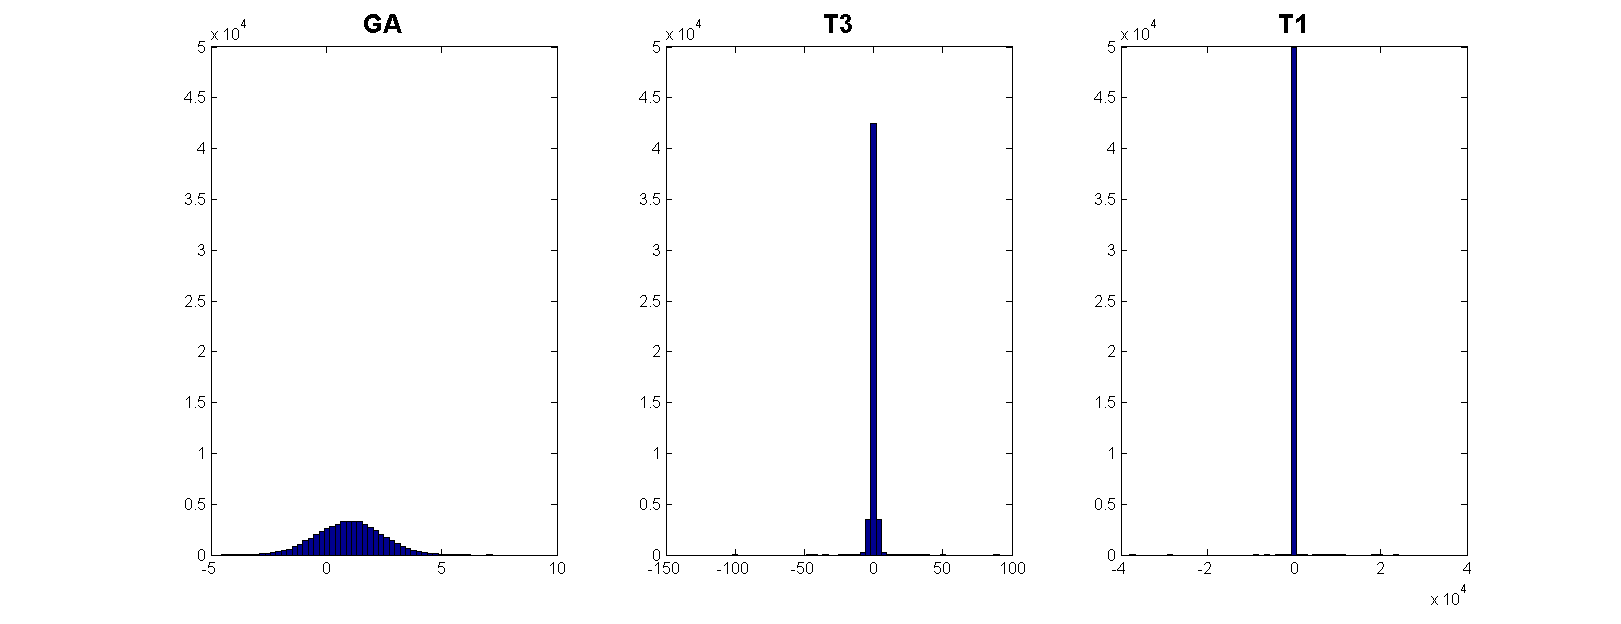
\includegraphics[width=.3\linewidth]{../Data_distributions.png}
	
	
	\end{pblock}
	
	\begin{pblock}{Leveraging in general}
	
	\end{pblock}
	
	\end{column}
    \begin{column}{.3\linewidth}


	\begin{pblock}{LS-based Distribution}	
	We wish to find the effect that a datapoint's class has on the predicted class for that datapoint.
	    \begin{equation}
	    \label{dyhatdy}
	    \frac{\delta \hat{Y}_n}{\delta Y_n}
	    \end{equation}
	There is a closed form solution which is linear in $y$
		\begin{equation*}
			\hat{\beta}_{OLS} = \left( X^T X \right)^{-1} X^T y
		\end{equation*}
	And prediction is also linear
		\begin{equation*}
			\hat{Y}_n = X_n*\hat{\beta}
		\end{equation*}
	Therefore \eqref{dyhatdy} is the coefficient
		\begin{equation*}
			\frac{\delta \hat{Y}_n}{\delta Y_n} = X \left( X^T X \right)^{-1} X^T
		\end{equation*}
	
	\end{pblock}

	\begin{pblock}{Test results}
	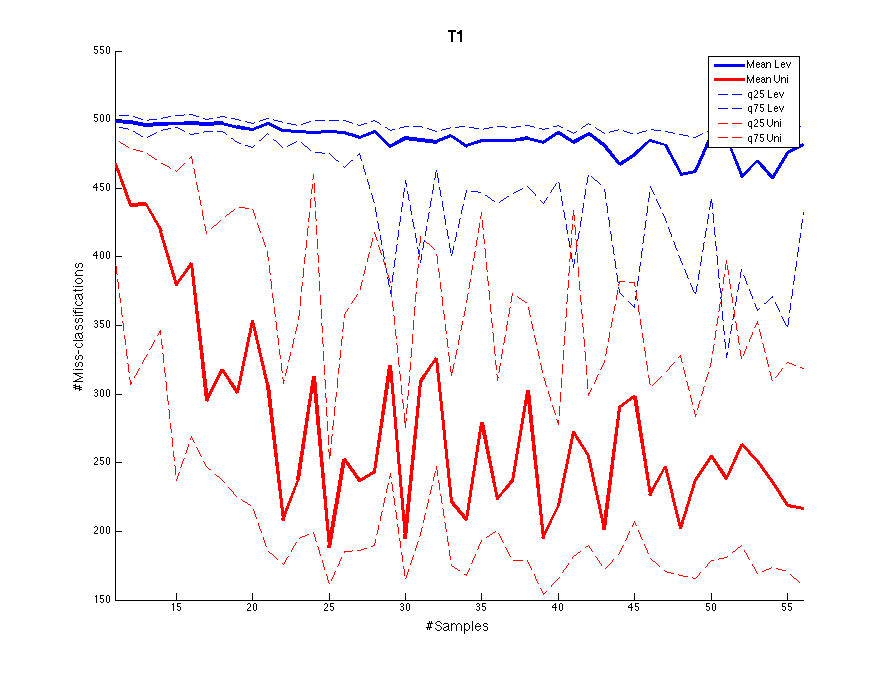
\includegraphics[width=\linewidth]{T1.png}
	N=1000 p=10
	\end{pblock}

	
	
    \end{column}
    \begin{column}{.3\linewidth}
    
    
    	\begin{pblock}{Sensitivity Based Distribution}
    	The target is again \eqref{dyhatdy} 
    	\begin{equation*}
    	\label{optimum}
    	 \hat{Y}_n = p(y|\bar{x},\bar{w}) \quad \bar{w} \  \text{s.t.} \ \frac{\delta L}{\delta\bar{w}}=0
    	\end{equation*}
    	Since \ref{optimum} depends both directly and indirectly on $y$ we see that
    	\begin{eqnarray*}
    	&\frac{\delta}{\delta y} \frac{\delta L}{\delta w} = 0\\
    	\Downarrow & \\
    	&\frac{\delta^2 L}{\delta y \delta \bar{w}} + \frac{\delta^2 L}{\delta \bar{w} \delta \bar{w}^T} \frac{\delta \bar{w}}{\delta y}= 0
    	\end{eqnarray*}
    	
    	and from this we can get our leverage score \eqref{dyhatdy}
    	
    	\begin{equation*}
    	\frac{\delta p(y|\bar{x}_n,\bar{w})}{\delta \bar{w}^T} \frac{\delta \bar{w}}{\delta y} = - \frac{\delta p(y|\bar{x}_n,\bar{w})}{\delta \bar{w}^T} \left[ \frac{\delta^2 L}{\delta \bar{w} \delta \bar{w}^T} \right]^{-1} \frac{\delta^2 L}{\delta y \delta \bar{w}}
    	\end{equation*}
    	\end{pblock}
    	
    
    \begin{pblock}{Uncertainty Based Distribution}
    	bla
    	\end{pblock}
    
    
    \end{column}
  \end{columns}
\begin{columns}
	\begin{column}{.61\linewidth}
		\begin{block}{Process}
			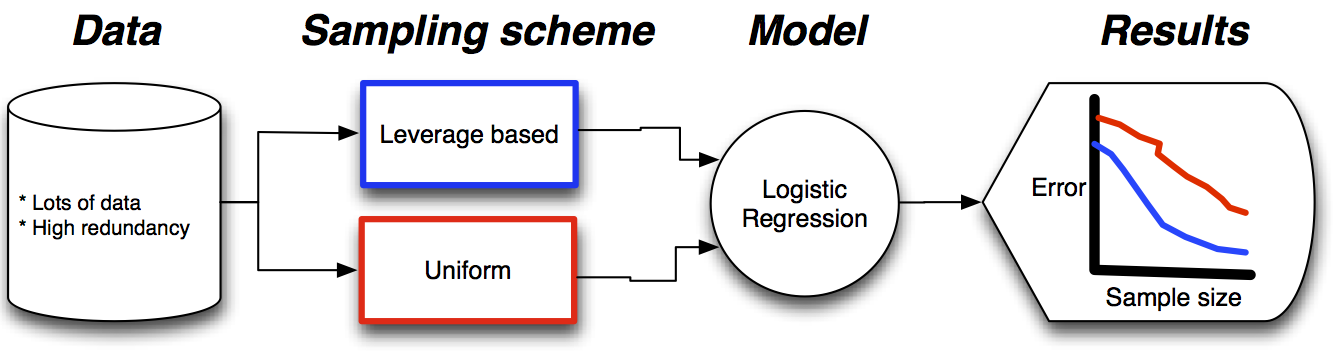
\includegraphics[width=\linewidth]{ThoughModel.png}
		  
		\end{block}
	\end{column}
	\begin{column}{.3\linewidth}
			\begin{block}{Conclusion}
				itr doesnt work because the classification doesnt gain much from the collective distribution of both classes.
			\end{block}
	\end{column}
\end{columns}	
	
  }
\end{document}